\section{实验结果分析}

\subsection{总体性能对比}
根据表\ref{tab:speedup}中加速比计算各方案在所有数据规模下的几何平均加速比,结果如下:
\begin{figure}[H]
    \centering
    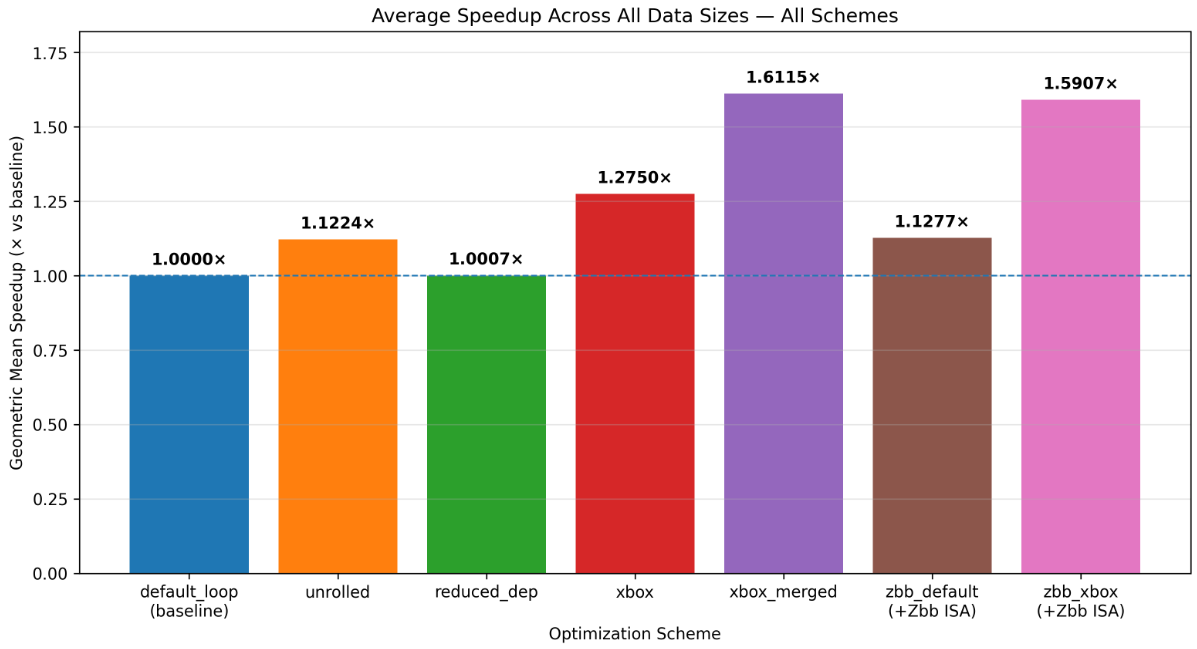
\includegraphics[width = 1\textwidth]{figure/speedup_avg.png}
    \caption{各优化方案在所有数据规模下的几何平均加速比}
    \label{fig:speedup_avg}
\end{figure}

从图\ref{fig:speedup_avg}可以看出,6种优化方案按照性能提升从低到高排序为:
\[
\texttt{reduced\_dep}<\texttt{unrolled}<\texttt{zbb\_default}
<\texttt{xbox}<\texttt{zbb\_xbox}<\texttt{xbox\_merged}
\]
其中，\texttt{xbox\_merged} 的几何平均加速比为 $1.6115\times$，是本实验中性能最优的实现；
\texttt{zbb\_xbox} 的几何平均加速比为 $1.5907\times$，略低于 \texttt{xbox\_merged}；
\texttt{reduced\_dep} 的几何平均加速比仅为 $1.0007\times$，与基线版本几乎相同。 

实验结果表明，不同优化方案的效果存在明显差异。相比局部的指令级调整，
将 SM4 轮函数中的部分计算转化为预计算查表操作能够获得更加显著的性能提升。

\subsection{查表优化为何有效} 查表优化包括 \texttt{xbox} 和 \texttt{xbox\_merged} 两种方案。
两种方案均利用了 SM4 线性变换的可加性，将部分运行时计算转化为预计算结果的组合。 
需要说明的是，\texttt{xbox} 并不是为完整的 $32$ bit 轮函数建立查找表。
完整轮函数具有 $2^{32}$ 种输入，不适合直接全部预计算。
实际做法是：针对单个字节经过 S 盒替换和线性变换后的贡献，建立一张包含 $256$ 个表项的查找表，再将 $4$ 个字节对应的结果进行组合。 
以 $1$ MB 输入规模为例，三种方案的吞吐率如下： 
\begin{table}[H] 
    \centering 
    \caption{1 MB 输入规模下查表优化方案的吞吐率对比} 
    \label{tab:xbox-throughput} 
    \begin{tabular}{c|c|c} 
        \toprule 方案 & 吞吐率（MB/s） & 相对基线提升 \\ 
        \midrule \texttt{default\_loop} & 21.755 & -- \\ 
        \texttt{xbox} & 27.738 & 27.50\% \\ 
        \texttt{xbox\_merged} & 34.927 & 60.55\% \\ 
        \bottomrule 
    \end{tabular} 
\end{table} 
        \texttt{xbox} 
        方案通过查表减少了运行时的 S 盒替换、字节组合和循环移位相关操作，使吞吐率由 21.755 MB/s 提升至 27.738 MB/s。 
        在此基础上，\texttt{xbox\_merged} 进一步建立 $4$ 张预旋转查找表，旋转偏移分别为 $0$ bit、$8$ bit、$16$ bit 和 $24$ bit。
        每张表包含 $256$ 个 $32$ bit 表项，占用 $1$ KB 空间，总空间开销为 $4$ KB。
        程序在初始化阶段完成表项计算，进入加密过程后只需查表并完成异或组合，不再执行额外的运行时循环移位。 
        从几何平均加速比看，\texttt{xbox\_merged} 相较 \texttt{xbox} 又提升了约 26.39\%。这说明在当前 RISC-V 开发板上，以少量额外存储空间换取消除运行时旋转操作具有较高收益。

\subsection{微架构优化的有限效果}

\subsubsection{循环展开(unrolled)}

\texttt{unrolled}方案通过将SM4的32轮迭代在编译阶段展开为32段顺序代码,减少了循环计数器自增、条件判断和分支跳转带来的额外开销。实验结果显示,\texttt{unrolled}方案在全部数据规模下的几何平均加速比为$1.1224\times$,即相较默认循环版本提升约12.24\%。

该方案能够带来稳定收益,但提升幅度仍然有限。原因在于:

\begin{itemize}
    \item SM4的主要计算开销仍然集中在每轮迭代中的S盒替换、线性变换和状态更新。循环展开只能减少循环控制开销,无法消除轮函数本身的核心计算;
    \item 循环展开会增大代码体积,但开发板每核心具有32 KiB的L1指令缓存。结合实验结果来看,代码展开后并未出现明显的性能下降,说明增加的代码规模尚未对整体性能产生显著负面影响;
    \item 因此,循环展开适合作为一种较为稳定的基础优化方式,但难以单独突破SM4轮函数自身的计算瓶颈。
\end{itemize}

\subsubsection{降低指令依赖(reduced\_dep)}

\texttt{reduced\_dep}方案尝试通过重排异或操作来缩短原始表达式中的依赖链。默认实现中的连续异或表达式为:

\[X_1 \oplus X_2 \oplus X_3 \oplus rk[i]\]

优化后将其拆分为两个可以独立计算的中间结果:

\[tmp_1 = X_1 \oplus X_2\]

\[tmp_2 = X_3 \oplus rk[i]\]

\[tmp = tmp_1 \oplus tmp_2\]

理论上,这种改写可以增加指令级并行机会,减少连续异或之间的串行依赖。然而实验结果显示,\texttt{reduced\_dep}方案的几何平均加速比仅为$1.0007\times$,与默认循环版本基本相同。在256 KB及以上输入规模下,其加速比甚至略低于$1.00\times$。

这一现象可能由以下原因共同导致:

\begin{itemize}
    \item 异或操作本身开销较低,并不是SM4轮函数中的主要性能瓶颈。相比之下,S盒访问和线性变换对整体运行时间的影响更加显著;
    \item 在\texttt{-O2}优化级别下,编译器已经能够对简单异或表达式进行一定程度的重排和寄存器分配优化,因此手工拆分表达式能够提供的额外收益较小;
    \item 新增的中间变量可能改变编译器的寄存器分配和指令调度结果,从而抵消理论上的依赖链缩短收益;
    \item 当输入规模增大时,流式数据访问和系统运行状态对总时间的影响更加明显,微小的局部优化容易被这些额外开销稀释。
\end{itemize}

因此,\texttt{reduced\_dep}方案说明:理论上可以增加并行机会的局部代码重排,并不一定能够转化为可观测的整体性能提升。优化效果仍然取决于编译器行为、关键路径位置和具体硬件执行特征。



\subsection{ISA扩展的独立与叠加效应}

RISC-V Zbb位操作扩展提供了多种适合密码算法实现的位操作指令。其中,与本实验中SM4实现关系较为密切的指令包括:

\begin{itemize}
    \item \texttt{rev8}:用于简化字节序反转操作。SM4按照大端序读取和输出32位字,而RISC-V开发板采用小端序存储。未启用Zbb扩展时,字节序转换通常需要多次加载、移位和或运算;启用Zbb扩展后,编译器可以使用更紧凑的字节反转指令序列;
    \item \texttt{rori}:用于简化循环移位操作。默认实现中的线性变换需要多次循环左移,通常可拆解为移位与或运算的组合;启用Zbb扩展后,编译器可以使用旋转类指令减少相关指令开销。
\end{itemize}

需要说明的是,Zbb扩展带来的实际收益不仅取决于指令集本身,还取决于编译器是否能够识别相应代码模式并生成合适的目标指令。因此,本实验通过对比不同编译配置下的实测结果评价其整体效果。

\subsubsection{独立应用Zbb扩展}

\texttt{zbb\_default}方案与\texttt{default\_loop}方案采用相同的32轮循环结构,区别在于编译时启用了Zbb相关扩展。两种方案的对比如下:

\begin{table}[H]
    \centering
    \caption{独立应用Zbb扩展前后的性能对比}
    \label{tab:zbb-independent}
    \begin{tabular}{c|c}
        \toprule
        方案 & 几何平均加速比 \\
        \midrule
        \texttt{default\_loop} & $1.0000\times$ \\
        \texttt{zbb\_default} & $1.1277\times$ \\
        \bottomrule
    \end{tabular}
\end{table}

实验结果显示,\texttt{zbb\_default}相对于基线版本取得了$1.1277\times$的几何平均加速比,即整体性能提升约12.77\%。

这一结果说明,Zbb扩展能够通过优化字节序转换和循环移位等局部操作带来稳定收益。但其提升幅度仍然明显低于\texttt{xbox}和\texttt{xbox\_merged}等查表方案。这表明局部指令替换可以减少部分执行开销,但无法从根本上改变SM4轮函数的计算结构。

值得注意的是,\texttt{zbb\_default}的性能与循环展开方案\texttt{unrolled}较为接近。两者的几何平均加速比分别为$1.1277\times$和$1.1224\times$。这说明在当前开发板上,减少局部位操作开销与减少循环控制开销能够获得相近幅度的性能收益。

\subsubsection{叠加应用Zbb扩展}

\texttt{zbb\_xbox}方案在四张合并查找表的基础上进一步启用了Zbb扩展。为了分析Zbb扩展在查表优化完成后是否仍然具有明显的边际收益,应当将其与\texttt{xbox\_merged}进行比较:

\begin{table}[H]
    \centering
    \caption{合并查表方案启用Zbb扩展前后的性能对比}
    \label{tab:zbb-combined}
    \begin{tabular}{c|c}
        \toprule
        方案 & 几何平均加速比 \\
        \midrule
        \texttt{xbox\_merged} & $1.6115\times$ \\
        \texttt{zbb\_xbox} & $1.5907\times$ \\
        \bottomrule
    \end{tabular}
\end{table}

实验结果显示,\texttt{zbb\_xbox}并未超过\texttt{xbox\_merged},其几何平均加速比反而低约1.29\%。这说明在合并查表优化完成后,Zbb扩展没有表现出可观测的额外正向收益。

其原因在于,\texttt{xbox\_merged}已经将四个字节位置对应的旋转结果预先存入四张查找表。预旋转操作在首次调用时的初始化阶段完成,加密主循环中只需执行查表和异或组合。因此,\texttt{rori}等旋转类指令在主循环中已经缺少进一步发挥作用的空间。

在该方案中,Zbb扩展仍可能优化分组加载和输出过程中的字节序转换,但这部分开销相对于32轮查表计算较小。同时,最终性能还会受到编译器指令选择、寄存器分配、代码布局和缓存访问行为等因素影响。因此,\texttt{zbb\_xbox}略低于\texttt{xbox\_merged}并不意味着Zbb扩展本身必然产生负优化,而是说明其边际收益已经非常有限,并可能被其他微小波动抵消。

综上,Zbb扩展适合用于优化默认循环实现,能够带来约12.77\%的稳定提升;但在合并查表方案已经消除大部分运行时旋转操作后,Zbb扩展与查表优化之间存在功能重叠,继续叠加的收益并不明显。由此可见,多种优化策略并不一定能够形成线性叠加效果。



\subsection{数据规模、缓存与局部性}

图~\ref{fig:speedup_trend}展示了各优化方案的吞吐率随输入数据规模变化的趋势。

\begin{figure}[H]
    \centering
    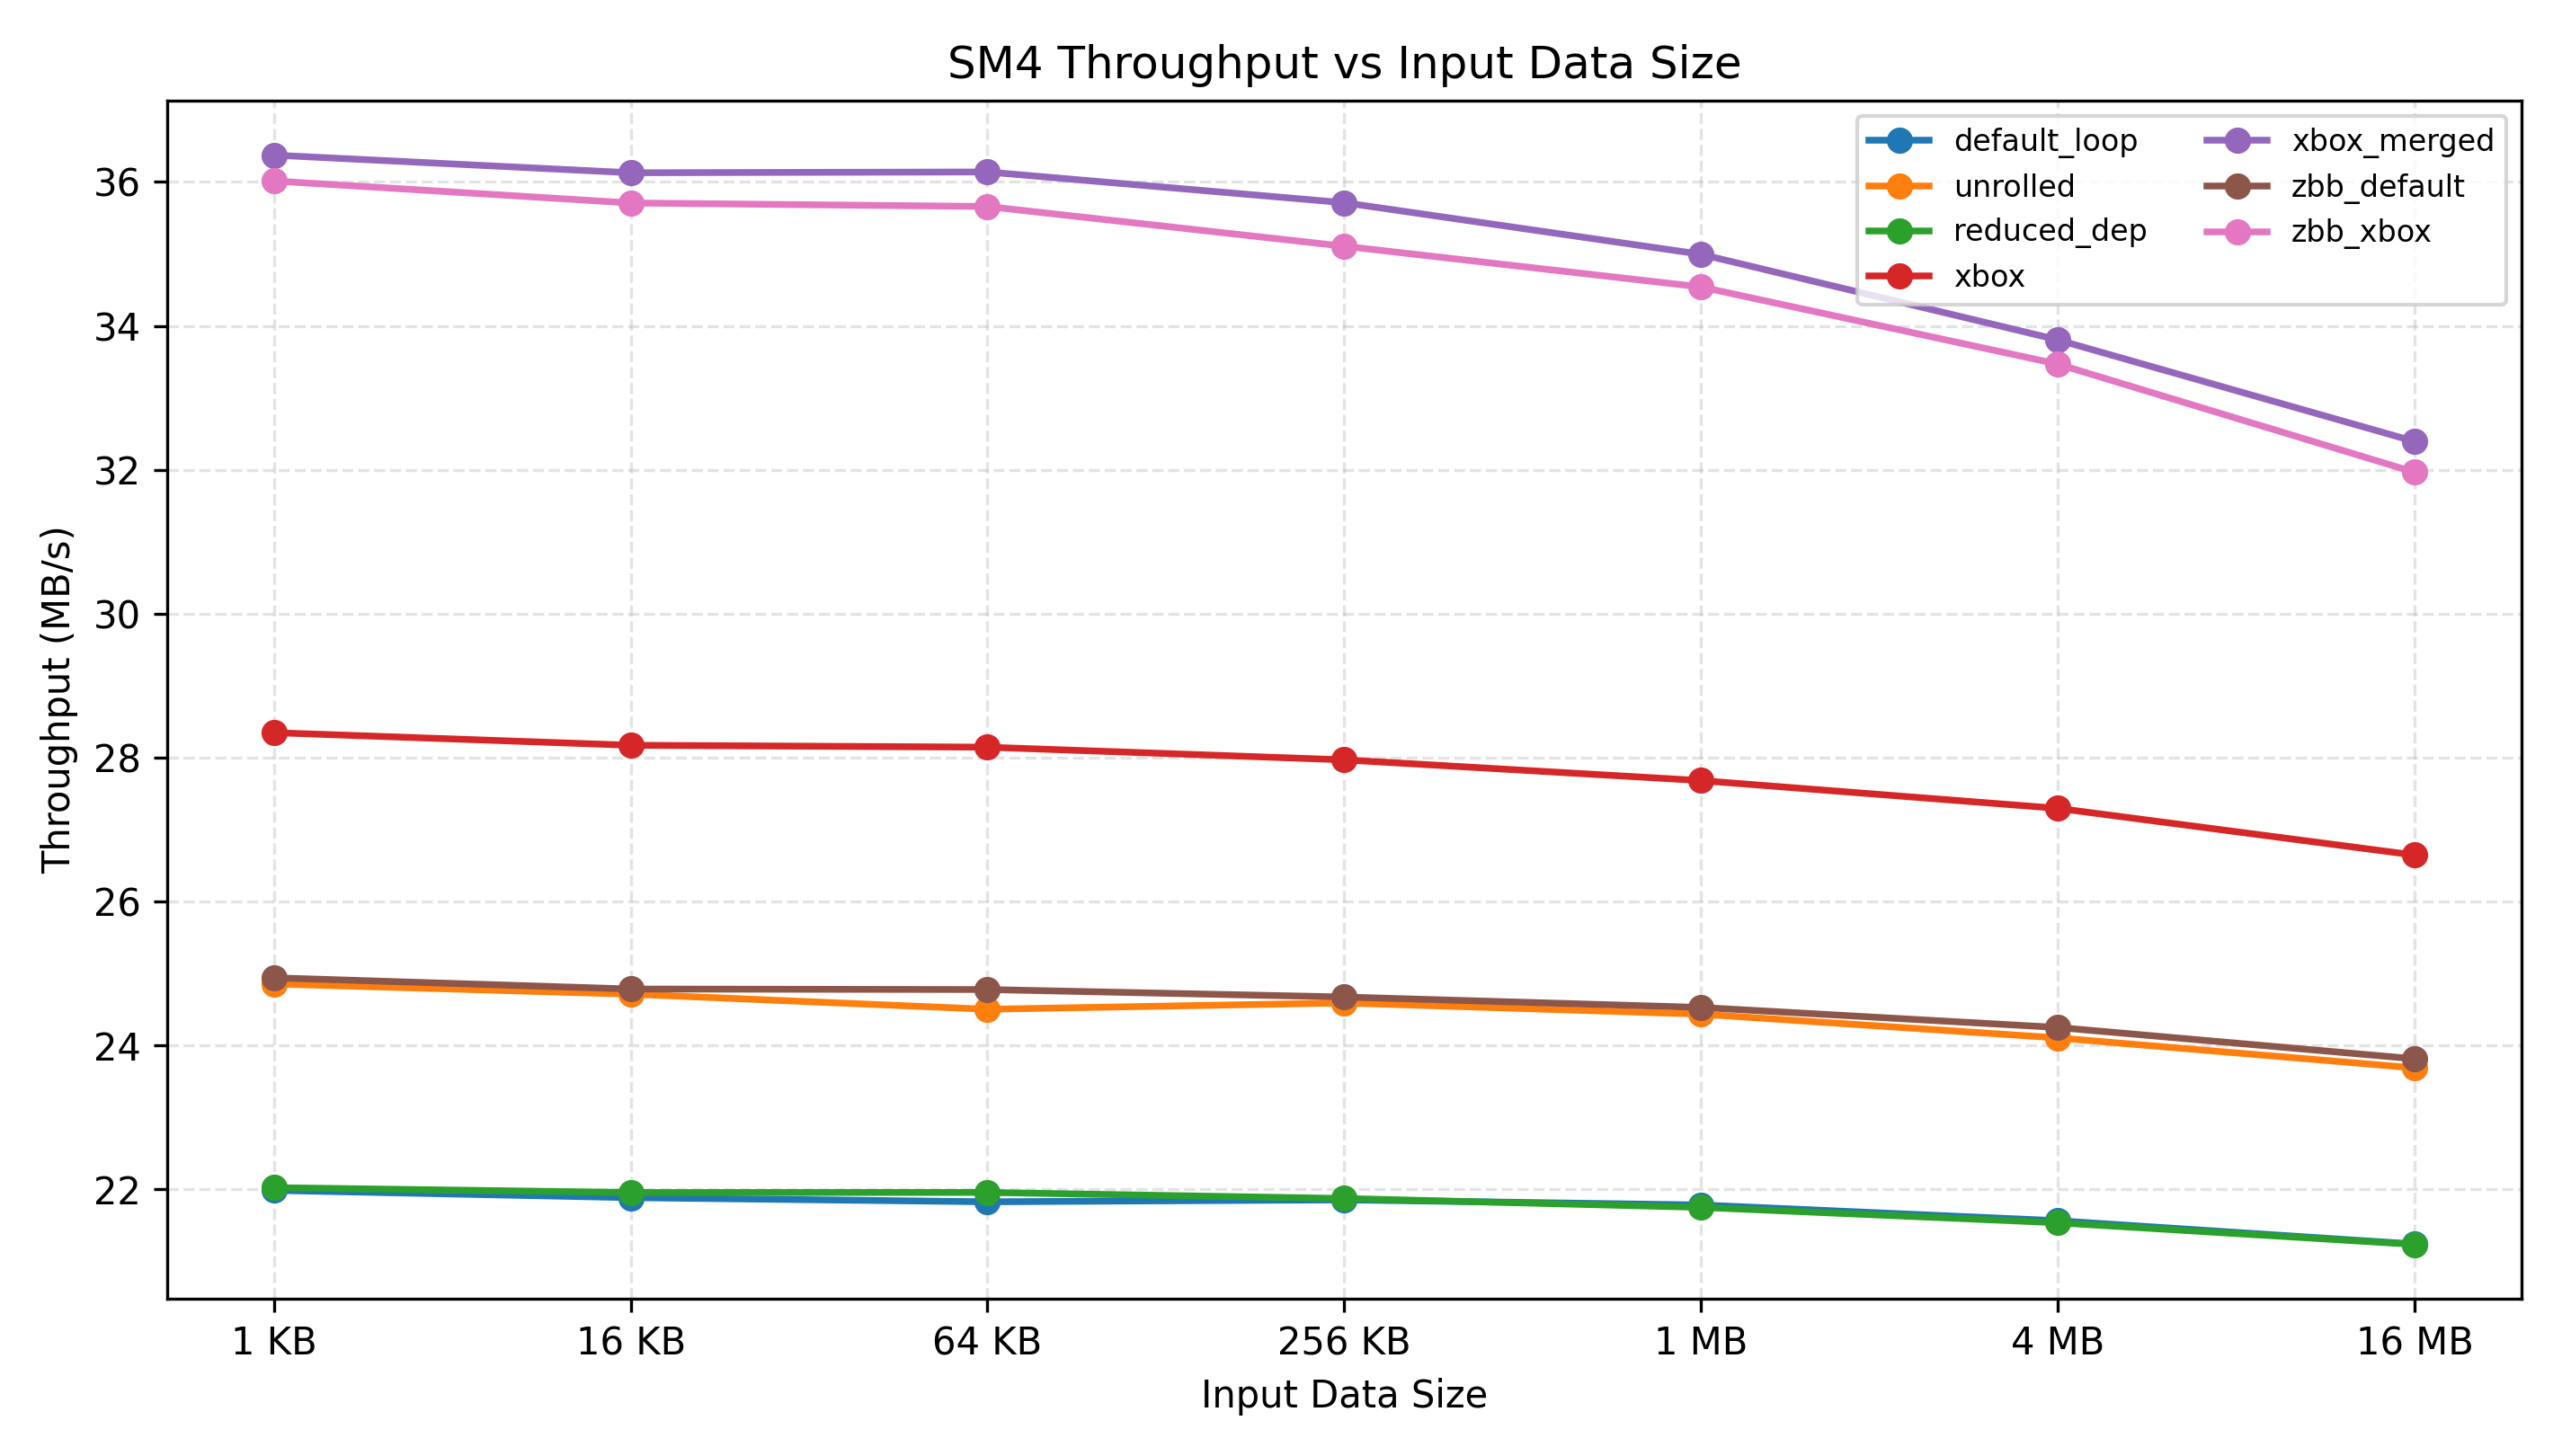
\includegraphics[width=1\textwidth]{figure/speedup_lines.png}
    \caption{各方案吞吐率随输入数据规模变化的趋势}
    \label{fig:speedup_trend}
\end{figure}

结合图~\ref{fig:speedup_trend}、表~\ref{tab:throughput}和表~\ref{tab:speedup},可以观察到以下两个趋势。

\begin{enumerate}
    \item \textbf{各方案的吞吐率均随输入规模增大而有所下降。}

    以默认循环方案\texttt{default\_loop}为例,吞吐率从1 KB输入规模下的21.949 MB/s下降至16 MB输入规模下的21.183 MB/s,下降约3.49\%。

    查表方案的下降幅度更加明显。
    例如,
    \begin{itemize}
        \item \texttt{xbox\_merged}的吞吐率从36.402 MB/s下降至32.243 MB/s,下降约11.43\%;
        \item \texttt{zbb\_xbox}的吞吐率从35.998 MB/s下降至31.794 MB/s,下降约11.68\%。
    \end{itemize}

    \item \textbf{多数优化方案的加速比随输入规模增大而逐渐减小。}

    其中,
    \begin{itemize}
        \item \texttt{xbox\_merged}的加速比从1 KB输入规模下的$1.6585\times$下降至16 MB输入规模下的$1.5221\times$;
        \item \texttt{zbb\_xbox}则从$1.6401\times$下降至$1.5009\times$。
    \end{itemize}
    

    相比之下,\texttt{unrolled}、\texttt{zbb\_default}和\texttt{reduced\_dep}等局部指令级优化方案的变化幅度较小。这说明查表方案虽然能够显著减少计算开销,但其相对优势会随着输入规模增大而有所减弱。
\end{enumerate}

\begin{figure}[H]
    \centering
    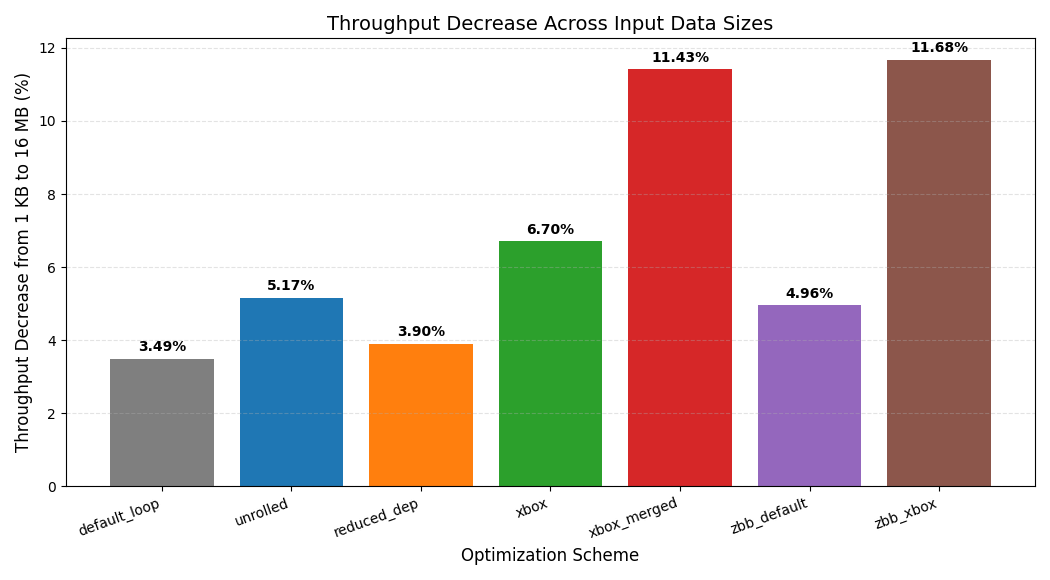
\includegraphics[width=0.9\textwidth]{figure/throughput_decrease.png}
    \caption{各方案从1 KB到16 MB的吞吐率下降比例}
    \label{fig:throughput_decrease}
\end{figure}

上述现象可以结合局部性原理进行解释。

对于\texttt{xbox\_merged}方案,四张预计算查找表共占用4 KB空间。查找表会在每个明文分组和每轮加密中被反复访问,因此具有较强的时间局部性。开发板每核心具有32 KiB的L1数据缓存,从容量上看,4 KB查找表具备驻留高速缓存的条件。

另一方面,输入数据按照分组顺序读取,具有较好的空间局部性,但单个明文分组处理完成后通常不会立即再次访问,因此时间局部性较弱。随着输入规模从1 KB增长至16 MB,流式数据加载与写回开销在总运行时间中的占比逐渐增加,从而稀释了计算优化带来的相对收益。

需要指出的是,仅凭吞吐率和加速比曲线无法直接证明Cache缺失次数显著增加。更加严谨的结论是:大规模输入下的性能衰减可能与缓存层次结构、流式数据访问开销和系统运行状态共同相关。若进一步使用硬件性能计数器统计L1 Cache miss、L2 Cache miss和内存访问次数,可以更加准确地区分不同因素的影响。



\section{实验总结}

综合以上实验结果与分析,可以得到以下结论:

\begin{enumerate}
    \item \textbf{预计算查表是本实验中效果最显著的软件优化方式。}
    
    \texttt{xbox}方案通过预计算单字节对轮函数的贡献,取得了$1.2750\times$的几何平均加速比;\texttt{xbox\_merged}进一步使用4张预旋转查找表消除运行时循环移位操作,几何平均加速比达到$1.6115\times$,为本实验中性能最优的方案。这说明对于SM4轮函数,采用空间换时间的方式减少运行时计算具有较高收益。

    \item \textbf{局部指令级优化能够带来稳定但有限的性能提升。}
    
    循环展开方案\texttt{unrolled}和启用Zbb扩展的\texttt{zbb\_default}分别取得了$1.1224\times$和$1.1277\times$的几何平均加速比。相比之下,\texttt{reduced\_dep}的几何平均加速比仅为$1.0007\times$,几乎没有可观测收益。这说明局部代码重排或指令替换是否有效,取决于其是否真正作用于程序的关键路径。

    \item \textbf{不同优化策略叠加后并不一定产生线性增益。}
    
    \texttt{zbb\_xbox}在合并查表方案的基础上进一步启用了Zbb扩展,但其几何平均加速比为$1.5907\times$,略低于\texttt{xbox\_merged}的$1.6115\times$。原因在于合并查表已经消除了大部分运行时循环移位操作,使\texttt{rori}等位操作指令能够继续发挥作用的空间明显缩小。因此,优化策略之间可能存在功能重叠,实际效果还会受到编译器指令选择、寄存器分配和缓存访问行为等因素影响。

    \item \textbf{输入规模增大后,各方案吞吐率均有所下降。}
    
    其中,\texttt{default\_loop}从1 KB到16 MB的吞吐率下降约3.49\%,而\texttt{xbox\_merged}和\texttt{zbb\_xbox}分别下降约11.43\%和11.68\%。这说明查表方案虽然在全部测试规模下仍保持明显优势,但对输入规模变化更加敏感。该现象可能与缓存层次结构、流式数据加载与写回开销以及系统运行状态共同相关。

    \item \textbf{工程实现中应综合考虑性能收益与资源开销。}
    
    \texttt{xbox\_merged}需要额外存储4张查找表,空间开销为4 KB。对于本实验使用的Orange Pi RV2开发板,每核心具有32 KiB的L1数据缓存,因此该额外开销处于可接受范围。在类似资源条件下,建议优先采用\texttt{xbox\_merged}方案;在缓存和存储空间更加受限的平台上,则应根据实际资源约束在性能与空间之间进行权衡。
\end{enumerate}

